\begin{figure*}
\label{fig:lightweight_breaks}
\centering
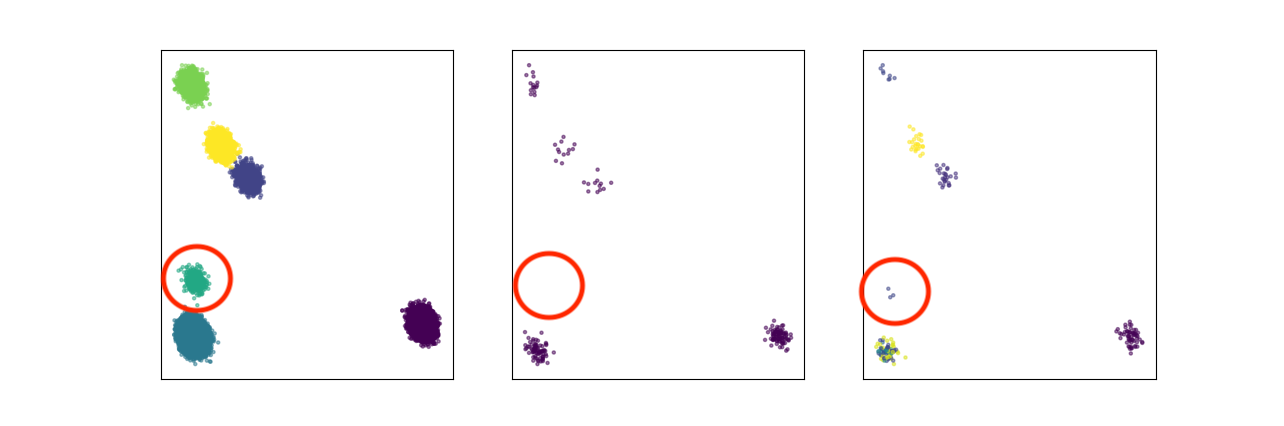
\includegraphics[width=.95\linewidth]{images/lightweight_breaks.png}
\caption{
The results of lightweight and fast-coreset constructions on a dataset of $n=100K$ points with clusters of varying size. The circled cluster has $\sim 400$ points. Coresets have 200 points.
\emph{Left}: Original multivariate-Gaussian dataset. \emph{Middle}: Lightweight coresets fail to capture the cluster of $\sim$400 points.
\emph{Right}: The Fast-coreset construction identifies all of the clusters.
}
\end{figure*}
